\section{Estructura del Funcionamiento}
\begin{frame}
    \begin{columns}[t]
        \begin{column}{.5\textwidth}
          \tableofcontents[sections={1-2},currentsection]
        \end{column}
        \begin{column}{.5\textwidth}
          \tableofcontents[sections={3-4},currentsection]
        \end{column}
    \end{columns}
\end{frame}

\subsection{Cálculos previos}
\begin{frame}[fragile]{Cálculos previos}
  Antes de realizar las primeras búsquedas se construye un objeto asociado a nuestra base de documentos

\end{frame}
\begin{frame}[fragile]{Almacenando Datos}
Se crea una estructura que relaciona cada palabra y los documentos
en los que aparece, y a su vez relaciona estos con las posiciones en
las que aparece cada palabra en dicho documento.

\pause

Para esto se usa un diccionario de diccionarios.
\end{frame}

\begin{frame}[fragile]{Alamcenando Datos}
Se crea cada vector documento, calculando el
tf-idf de cada palabra con funciones que estan implementadas dentro de una
clase TfIdfDirectory, de forma muy sencilla.
\pause

\begin{figure}[h]
    \center
    \includegraphics[width=10cm]{RepresentacionDelPreCalculo.png}
    \caption{Precálculo}
\end{figure}

\end{frame}

\subsection{Búsquedas}
\begin{frame}{Haciendo Búsquedas}

Cuando se introduce una búsqueda, esta se convierte en un vector ndimensional,
y se calcula su similitud coseno con todos los vectores documento.
Luego se seleccionan los 5 documentos de mayor similitud y se devuelven
como resultado.
\pause

\begin{figure}[h]
    \center
    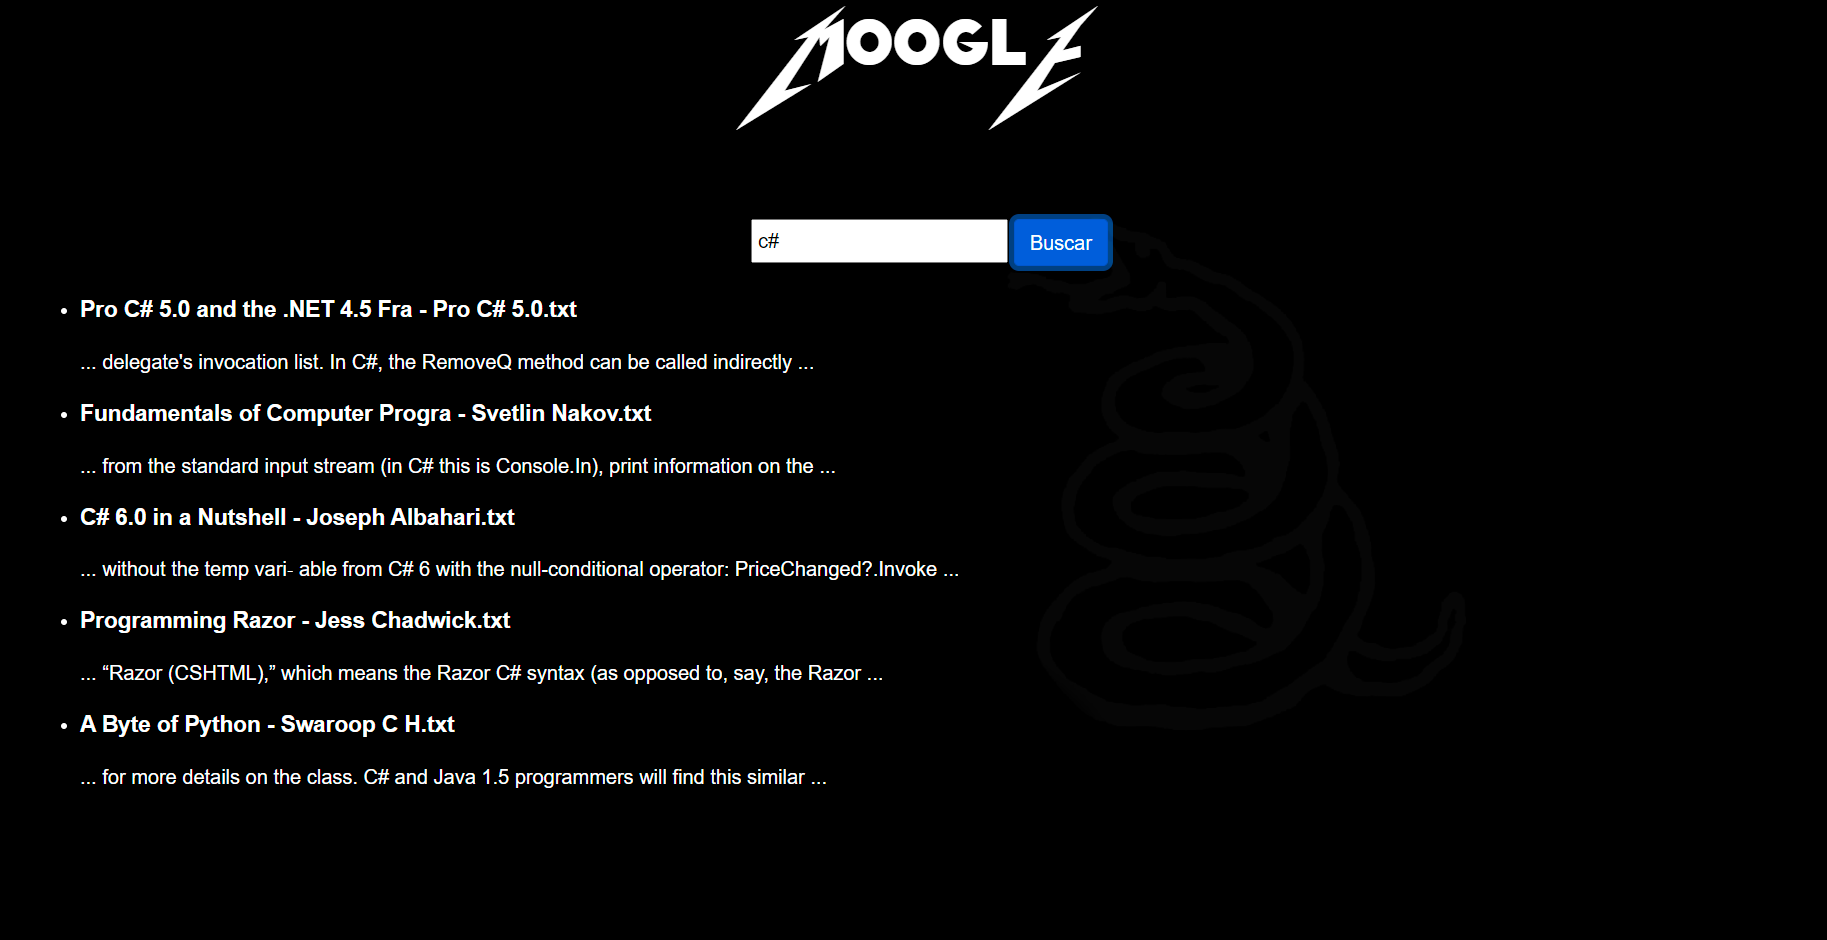
\includegraphics[width=6cm]{busqueda.png}
    \caption{Ejemplo de una búsqueda}
\end{figure}

\end{frame}

\begin{frame}[fragile]{Haciendo Búsquedas}

\begin{figure}[h]
    \center
    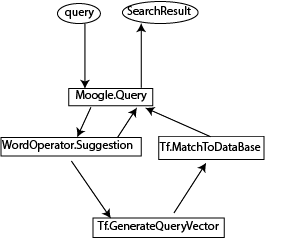
\includegraphics[width=7cm]{DiagramaDeClases.png}
    \caption{Proceso de respuesta}
\end{figure}

\end{frame}
